\chapter{Introduction}
\label{chapter1}
This chapter gives an outline of the important developments and difficulties in the transport
and energy sectors that form the basis for this research. Section \ref{sec:motivation} motivates the work being presented. Then, Section \ref{sec:contributions} enumerates its research objectives and contributions. Next, Section \ref{publications} lists the publications emanating from the research contributions. Finally, Section \ref{structure} discusses the structure of the document. This chapter gives an outline of the important developments and difficulties in the transport and energy sectors that form the basis for this research.

\section{Motivation}
\label{sec:motivation}

% \begin{figure}[htbp]
%     \centering
%     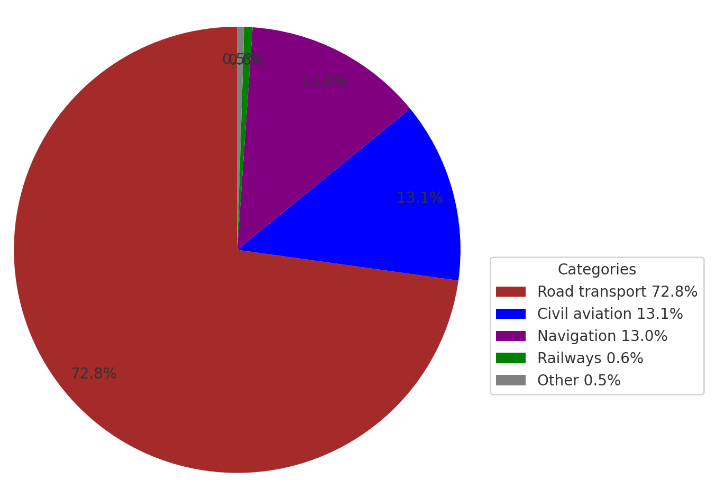
\includegraphics[scale=0.55]{Crest/Images/ghg_stats.png}
%     \caption{Greenhouse gas emissions from transport by mode 2014-20 \cite{alfaseeh2019multi}}
%     \label{fig:ghg_stats}
% \end{figure}
Recent data has shown that between the years 1890 and 2008, the temperature in Ireland. 
has grown by 0.7 degree Celsius. It has changed the growing season, affecting farming, and
has increased the number of animals suited to warmer temperatures. Data trends show an
increase in the frequency and impact of storms in the last few decades \cite{alfaseeh2019multi}. Similar situations are being seen all over the world (such as China, India, Mexico, Brazil just to name a few countries). Indeed, up to 2021, Bhutan is the only carbon-neutral country in the world where the daily operation of the country does not cause lasting damage to the environment \cite{europeancommission2024promoting}. As a way to fight these growing climate threats, the European Union (EU) and the European Commission have presented a package of measures designed to make Europe the first climate-neutral continent in the world by 2050. Some of the critical components of this policy include cutting emissions, preserving the natural environment and investing in cutting edge research and innovation \cite{shariff2022state} . This European Green Deal is the long-term strategy of the EU to protect humans, animals and plants by cutting pollution and securing a healthy planet for generations to come \cite{greendeal}.

The transportation sector has been identified as a key area to undergo significant
transformation as a result of the aforementioned Green Deal. In the last decade there has
been growing awareness about the hazardous effects of logistic activities, such as
transportation, which has a considerable impact on the ecological environment, and
therefore requests for more environmentally friendly practices. The EU has targeted a 40\%
reduction in Green House Gas (GHG) emissions by 2030 with respect to the levels of 1990
\cite{europeancommission2024promoting}. According to the European Environment Agency, this is a challenge for the transportation sector, which is responsible for 20\% of total GHG emissions. Furthermore, according to the 2019 report of the world energy outlook series, the future estimation of energy systems indicates that a severe loss in available amounts of fossil energy will happen by 2040 \cite{greendeal}. Therefore, electrification and autonomy of the transportation systems are viewed as a critical avenue to achieving the ambitions as set-out in the EU Green Deal.

The operation of transportation networks through (increasingly Autonomous) Electric
Vehicles (AEVs) fleets requires also a profound change in the energy sector, where the use
of Renewable Energy Sources (RES) must become the norm \cite{alfaseeh2019multi} \cite{baudru2024comparative} and decentralisation enables stability and flexibility of the grid (smart grid). This not only requires specific policies, but a general shift in mindset in terms of how to effectively manage this decentralised generation to effectively service the demands of end users and customers. The generation and availability of RES is volatile by nature and, instead of adapting it to current society demands, an emphasis must be placed on being more cognisant of the efficient use of every unit of energy required. In addition to large-scale wind and solar farms (which are typically managed at a national level), Smart Energy Communities (SECs) are decentralised clusters of energy users—such as households, businesses, or institutions—that are locally interconnected and capable of both generating and consuming RE. Typically supported by digital infrastructure and storage systems, SECs coordinate energy generation (e.g., via solar or wind), storage (e.g., through batteries), and demand within a geographically bounded area. By enabling distributed energy generation, peer-to-peer trading, and cooperative decision-making, SECs contribute to a more resilient, carbon-neutral grid. They represent a foundational model for the emergence of the term ‘Energy Citizen’, empowering individuals and communities to participate actively in the management of the electric power system, and thereby enhancing both its efficiency and sustainability.

In response to these imperatives, several strategies have been proposed, including the
adoption of RES \cite{gradisar2000enhancing}, advancements in vehicle technology [51], and the implementation of Intelligent Transportation Systems (ITS) \cite{wallar2019optimizing}. Within ITS, Ride-sharing has presented new opportunities for the SEC sector to be productive with energy usage \cite{agatz2012optimization}. Dynamic ride-sharing systems aim to match riders and drivers with similar itineraries and time schedules on short-notice \cite{soa_rideshare}. These systems can reduce the number of cars used for personal travel (improving the utilisation of available seat capacity) as well as the total distance for such travels, thus reducing the environmental impact.

Motivated by the aforementioned sustained mass transition to AEVs and by the distributed
energy generation and storage of local SECs, this PhD thesis presents the design, implementation
and evaluation of a carbon-neutral, community-based, scalable ride-sharing system. The
PhD thesis considers a future where a ride-sharing service must rely on a 100\% AEV fleet
operating solely on RES. Emphasis is placed on individual citizens (rather than on haulage
transportation) that collectively aim to minimise their impact on the environment through
the use of ride-sharing commutes powered by green energy sources. The ride-sharing
service entails an AEV fleet operating in a city that encapsulates multiple distributed SECs,
each of them producing RES over a time horizon, owning and operating a number of AEVs and charge stations. Each SEC sets out its available AEVs for ride-sharing based on the RES
energy generation that can be used to charge them.

The challenges to operate such a ride-sharing service include managing how the overall fleet of AEVs is distributed across the various SECs of a city. While each SEC initially deploys its own set of AEVs, the dynamic nature of ride-sharing operations and inter-SEC collaboration often requires a city-wide perspective, where the effective partitioning and reallocation of AEVs between SECs must be carefully coordinated, as well as the allocation of trip petitions (TPs) to AEVs, their routing and charging scheduling over a simulated time horizon. These challenges become even
more pronounced by the need to operate at scale (with large EV fleets across metropolitan
areas), in real-time (with the service processing the TPs as they arise), and under dynamic
resources (with the number of active AEVs depending on RES availability over time across
multiple locations). Finally, the distributed SECs are indeed inter-related, and therefore
enabling decentralised co-operation to optimise their resources.

All in all, the EU Green Deal targets 2050 to be energy-neutral, envisioning a sustained
transition from diesel-based transportation to AEVs, and from a traditional energy market to
a fully RES-based one. To enable this change, the transportation sector must demonstrate
leadership by accelerating the use of AEVs and SECs. This PhD thesis contributes to this vision for green transportation by providing a computational efficient, scalable, and environmentally sustainable ride-sharing service.


% Transportation is a major contributor to environmental degradation, accounting for 28\% of greenhouse gas (GHG) emissions and 20\% of total energy consumption in the United States alone \ref{fig:ghg_stats} \cite{alfaseeh2019multi}. Globally, the sector relies heavily on oil-based fuels, which are not only non-renewable but also highly polluting, exacerbating the climate crisis. The pressing need to reduce these emissions has prompted international frameworks such as the \textit{United Nations Sustainable Development Goals (SDGs)} \cite{shariff2022state} and the \textit{European Green Deal} \cite{europeancommission2024promoting}, which emphasise carbon neutrality as an essential—not optional—objective. The European Green Deal, for instance, aims to make Europe the first climate-neutral continent by 2050, prioritising the decarbonisation of energy-intensive sectors like transportation \cite{greendeal}.

% In response to these imperatives, several strategies have been proposed, including the adoption of RES \cite{gradisar2000enhancing}, advancements in vehicle technology \cite{hajari2021distributed}, and the implementation of \textit{Intelligent Transportation Systems (ITS)}\cite{wallar2019optimizing}. ITS has proven to be especially effective, optimising various transportation operations such as dynamic routing, traffic flow control, and energy-efficient vehicle scheduling\cite{fiedler2018impact}. By enhancing operational efficiency and reducing congestion, ITS significantly curbs fuel consumption and emissions \cite{alfaseeh2019multi} \cite{baudru2024comparative}.

% Recent years have seen a paradigm shift in the transportation sector, marked by the widespread adoption of \textit{electric vehicles (EVs)} and the rise of \textit{ride-sharing services}. While ride-sharing services reduce the number of vehicles on the road, lowering pollution and traffic congestion, integrating EVs into these systems provides further environmental benefits by replacing fossil fuel-based engines with zero-emission alternatives \cite{gradisar2000enhancing}. However, achieving large-scale adoption of EV-based ride-sharing services requires overcoming challenges such as:
% \begin{enumerate}
%     \item \textbf{Passenger-to-vehicle allocation:} Matching passengers to available vehicles in real time while minimising operational costs and maximising passengers served \cite{alonso2017ondemand} \cite{optimiserideshare} \cite{hasan2018community}.
%     \item \textbf{Vehicle routing:} determining the most energy-efficient routes that also account for passenger travel demands \cite{meng2021dynamic} \cite{ghandeharioun2023rideshare}.
%     \item \textbf{EV charging scheduling:} Ensuring efficient charging operations that minimise downtime \cite{song2023electric} \cite{satoya2014community} \cite{Reference104}.
% \end{enumerate}

% These challenges become even more pronounced as the scale of operations increases. Efficient algorithms must not only address the travel demands but also ensure scalability to support the deployment of large EV fleets across metropolitan areas.

% \subsection{Role of Smart Energy Communities (SECs)}

% SECs integrate RES, such as solar and wind, with smart grid technologies, enabling the localised production, distribution, and consumption of clean energy\cite{hildermeier2019smart}. Beyond their potential to reduce reliance on fossil fuels, SECs could be used as a solution to enable EV-based ride-sharing services. Specifically, they enable:
% \begin{itemize}
%     \item \textbf{Dynamic energy allocation:} Matching charging schedules to periods of high renewable energy availability\cite{hemavathi2022study}\cite{vanSummeren2019community}.
%     \item \textbf{Depot functionality:} Serving as depots for ride-sharing EVs.
%     \item \textbf{Collaborative operations:} Negotiating with other SECs to balance resources and maximise the number of trips served\cite{shariff2022state}.
% \end{itemize}

\section{Research Objectives and Contributions}
\label{sec:contributions}
The PhD thesis has the following 3 research objectives:

\subsection{Research Objective 1}
\textbf{A Carbon-Neutral, Community-Based, Reactive and Scalable Ride-Sharing Service.}
This research objective entails the design, implementation and evaluation of a ride-sharing service aligning with the ambition of the aforementioned EU Green Deal goals.

Specifically, the research objective leads to the following research contributions:
\begin{itemize}
    \item \textbf{Contribution 1:} The formulation of a ride-sharing simulation service that explicitly incorporates the conditions outlined above, namely the decentralised structure of SECs, dynamic TPs, RES integration, and the flexible allocation of AEVs, all operating with the goal of maximising TP fulfilment, presented as a variant of the classical Dynamic Vehicle Routing Problem with Time Windows \cite{vrp_survey}. The dynamic resources are provided
    by a number of SECs spread across a city, each of them owning a number of AEVs
    and using its own RES generation function to dynamically charge (and release) them
    over time. The dynamic requests are provided via TPs released over time,
    each of them with its own location and pick-up/drop-off times. The formulation of
    the ride-sharing service integrates energy generation, allocation and reactive re-
    routing constraints, with the objective function of maximising the overall number of
    TPs being served.

    \item \textbf{Contribution 2:} The design and implementation of a ride-sharing service, based on an algorithm following a reactive-based simulation approach on top of a greedy-based decision-making process. The algorithm favours scalability over optimality, therefore evaluating its applicability to real-world instances based on the transportation of large cities.

    \item \textbf{Contribution 3:} The development of a parameterised instance generator to align existing benchmarks (i.e. Google HashCode) and public datasets (i.e. NYC taxis) to the proposed problem formulation of Contribution 1. This is paired with the generation
    of a problem-specific benchmark for testing the performance of the solution approach of Contribution 2 under various configurations.     
\end{itemize}

\subsection{Research Objective 2}
\textbf{Decentralised Vehicle Allocation for Community-Based Ride-Sharing Services.}
This research objective extends Research Objective 1 by integrating the design,
implementation and evaluation of the vehicle fleet allocation to the ride-sharing service.

Specifically, the research objective leads to the following research contributions:
\begin{itemize}
    \item \textbf{Contribution 4:} The formulation of the vehicle allocation problem both as a centralised optimisation problem (using a MIP formulation) and as a decentralised one, using an iterative negotiation process among connected-SECs. On the latter, each SEC acts as an independent agent, and carries out a number of negotiations with any other SEC it is connected to over a simulated time horizon. In such negotiations, connected
    communities decide the potential exchange of AEVs among them, based solely on their local information. The criticality of the vehicle allocation problem lies on its co-
    operation with its underlying ride-sharing problem to ensure adequate AEV to TP
    matching and routing. Once a SEC allocated a fixed number of AEVs from the AEV
    fleet, it manages the TPs of its own neighbours by operating the ride-
    sharing solution approach of Contribution 2.

    \item \textbf{Contribution 5:} The implementation of the vehicle allocation problem, using a novel Multi-Objective and Multi-Agent Reinforcement Learning (RL) algorithm, involving Deep Q-Learning with Graph Convolutional Networks. The algorithm equips SECs with the ability to learn from previous-negotiations, enabling them to improve their decision-making as the simulated time horizon goes by.

    \item \textbf{Contribution 6:} The modification of the instance generator and problem benchmark of Contribution 3, for it to align to the problem formulation of Contribution 4, as well as its further measuring of the solution approach of Contribution 5 under different community connectivity-levels and transport request distributions.    
\end{itemize}

\subsection{Research Objective 3}
\textbf{Reward-based Charging Schedule for a Community-based Ride-sharing Service.}
This research objective extends Research Objective 1 by integrating the design,
implementation and evaluation of reward-based charging scheduling to the ride-sharing
service.

Specifically, the research objective leads to the following research contributions:
\begin{itemize}
    \item \textbf{Contribution 7:} The formulation of the reward-based charging schedule, where each SEC owns a number of Charging Stations (CSs), and its RES generated being split into (i) the energy used to release its own AEVs and (ii) the energy used to recharge already operative AEVs. The charging schedule exploits the inter-relation of SECs, enabling (1) host TPs to be served by an AEV of a different SEC, and (2) such AEVs to recharge their batteries in a host CSs in return.

    \item \textbf{Contribution 8:} The implementation of the reward-based charging schedule via a decision-making process accounting for different factors, including the proximity and waiting times of available CSs, the potential for service interruptions due to charging, and the dynamic re-allocation of AEVs based on real-time assessments of energy
    consumption and vehicle availability. Additionally, the algorithm incorporates the
    flexibility to modify charging schedules dynamically by considering the collective
    prospects of multiple AEVs.

    \item \textbf{Contribution 9:} The modification of the instance generator and problem benchmark of Contribution 3, for it to align to the problem formulation of Contribution 7, as well as its further measuring of the solution approach of Contribution 8 under various configurations.    
\end{itemize}

% \subsection{Contributions}
% This thesis makes the following key contributions:

% \begin{enumerate}
%     \item \textbf{A carbon-neutral, community-based, reactive, and scalable ride-sharing service tailored to SECs.} 
%     This service consists of a network of independent but interrelated SECs, each equipped with its own EVs and Trips Petitions(TPs). These SECs operate autonomously but are capable of collaborating with one another to maximise the number of trips served. It is built on an algorithmic framework for real-time vehicle allocation and routing, enabling dynamic responses to evolving transportation demands.
    
%     The scalability of the system is a key feature, supported by a parameterised instance generator that aligns with existing benchmarks such as Google HashCode and public datasets like the NYC taxi data. This generator enables the evaluation of the system across diverse operational configurations, such as variations in trip flexibility, fleet size, and community connectivity. The solution was shown to process up to 10,000 trip petitions in less than two minutes, demonstrating its capability to handle large-scale urban ride-sharing scenarios.
    
%     Real-world evaluations using the NYC taxi dataset revealed that the system reduced the number of vehicles required by 84\% compared to traditional private transport, significantly decreasing traffic and pollution. The additional travel distance incurred due to ride-sharing was reasonably small, at only 21\%. This result indicates that the proposed method achieves a good balance between minimising vehicle usage and ensuring reasonable travel times, making it well-suited for large-scale urban mobility systems.
    
%     \item \textbf{A decentralised vehicle allocation framework for community-based ride-sharing services.} 
%     In this framework, multiple independent SECs within a metropolitan area manage their transportation needs by competing for vehicle resources to serve TPs. The vehicle allocation problem is modelled using centralised and decentralised approaches to examine how varying levels of community connectivity—defined as the degree of communication and resource sharing between SECs—affect resource distribution and operational performance.
    
%     To solve this complex allocation challenge, a Multi-Objective and Multi-Agent Reinforcement Learning (RL) method was developed. This approach combines Deep Q-Learning with Graph Convolutional Networks (GCNs), enabling SECs to negotiate vehicle allocations based on historical performance and current operational needs. The decentralised structure allows SECs to make independent decisions while collaboratively optimising overall system performance. This approach directly builds on the foundational allocation and routing algorithm described in Contribution 1.
    
%     The framework was evaluated using public datasets, including NYC taxi data and Google HashCode, and demonstrated scalability for large instances with up to 10,000 trips processed in a few seconds. The results show that the framework efficiently distributes vehicles across SECs, leading to higher operational efficiency, as reflected in the increased number of trip petitions served in real-time.

%     \item \textbf{An intelligent charging scheduler for a proactive, community-based, carbon-neutral ride-sharing service.} 
%     Building on the allocation and routing algorithm from Contribution 1, this scheduler optimises the charging processes for EVs within the SECs while ensuring carbon neutrality through the exclusive use of renewable energy. The scheduler addresses critical operational challenges, including minimising EV downtime and ensuring sufficient availability of vehicles for ride-sharing operations.
    
%     The scheduler incorporates a proactive approach to align charging activities with renewable energy production and travel demand. This approach allows SECs to manage their EV fleets efficiently, reducing the impact of charging on TPs fulfilled and operational reliability. The results demonstrate that the scheduler significantly enhances fleet efficiency, as reflected by a higher number of trip petitions served while maintaining carbon-neutral operations.
    
%     Evaluations using public datasets, such as NYC taxi data and Google HashCode, confirmed the solution’s scalability and adaptability to real-world conditions. The scheduler balances frequent charging needs with travel demands. This contribution extends the framework’s applicability to large-scale urban systems by enabling integration of EV charging into the overall ride-sharing service.
    
% \end{enumerate}

\section{Publications}
\label{publications}
The PhD thesis has the following 3 publications:
\begin{enumerate}
    \item \textbf{Publication 1 - Research Objective 1: 
        A Carbon-Neutral, Community-Based, Reactive and Scalable Ride-Sharing Service.} \cite{smartgreens}.
         \begin{itemize}
             \item Authors: Nagarajan, A.; McGibney, A.; Fenton, P. and Castiñeiras, I.
             \item Venue: In Proceedings of the 12th International Conference on Smart
                   Cities and Green ICT Systems.
             \item Year: 2023.
             \item Link: \href{https://www.scitepress.org/PublicationsDetail.aspx?ID=tZN50XMYOaQ=&amp;t=1}{SCITEPRESS publication link}
             \item Acceptance Rate: 30\% for full-paper publications.
             \item Github: \ \url{https://github.com/Nasheor/reactive\_rideshare}   
         \end{itemize}

    \item \textbf{Publication 2 - Research Objective 2:
    Decentralised Vehicle Allocation for Community-Based Ride-Sharing Services} \cite{nagarajan2024decentralised}.
         \begin{itemize}
             \item Authors: Nagarajan, A.; McGibney, A.; Fenton, P. and Castiñeiras, I.
             \item Venue: Communications in Computer and Information Science (Volume 1989).
             \item Year: 2024.
             \item Link: \href{https://link.springer.com/chapter/10.1007/978-3-031-70966-1_2}{Springer publication link}
             \item Acceptance Rate: 33\% for full-paper publications.
             \item Note: The publication requested a 30\% of novelty with respect to Publication 1. Indeed, a 70\% of novelty is provided in the paper.
             \item Github:\ \url{https://github.com/Nasheor/Fleet_allocation}   
         \end{itemize}

    \item \textbf{Publication 3 - Research Objective 3:
    Reward-based Charging Schedule for a Community-based Ride-sharing Service.} \cite{rewardcharging}.
         \begin{itemize}
             \item Authors: Nagarajan, A.; McGibney, A.; Fenton, P. and Castiñeiras, I.
             \item Venue: In Proceedings of the 3rd International Conference on IEEE Smart Mobility.
             \item Year: 2024.
             \item Link: \href{https://ieeexplore.ieee.org/document/10733393}{IEEE publication link}
             \item Acceptance Rate: 51\% for full-paper publications.
             \item Note: The publication requested a 30\% of novelty with respect to Publication 1. Indeed, a 70\% of novelty is provided in the paper.
             \item Github:\ \url{https://github.com/Nasheor/EcoRideSchedule}   
         \end{itemize}
\end{enumerate} 

\section{Structure}
\label{structure}
The remainder of this PhD thesis is organised as follows:
\begin{itemize}
    \item Chapter \ref{chapter2} presents an analysis of the current body of work that serves as the foundation for the PhD thesis.

    \item Chapter \ref{chapter3} presents the research objective 1, with the design, implementation and evaluation of a ride-sharing service aligning with the ambition of the aforementioned EU Green Deal goals.

    \item Chapter \ref{chapter4} presents the research objective 2, with the design, implementation and evaluation of the vehicle fleet allocation integrated to the ride-sharing service.

    \item Chapter \ref{chapter5} presents the research objective 3, with the design, implementation and evaluation of the reward-based charging scheduling integrated to the ride-sharing service.

    \item Chapter \ref{chapter6} presents a summary of the findings and a discussion of potential future work.
\end{itemize}
